\documentclass{article}
\usepackage[
    % letterpaper,
    margin=1in,
    % headheight=13.6pt,
]{geometry}

%%%% Page Header and Foot %%%%
\usepackage{fancyhdr}
\fancypagestyle{plain}{
\fancyhf{}
\fancyhead[L]{ECE 14:332:226}
\fancyhead[C]{\textbf{Probability And Random Processes}}
\fancyhead[R]{Summer 2023}
\fancyfoot[L]{}
\fancyfoot[C]{\thepage}
\fancyfoot[R]{}
}
\pagestyle{plain}

%%%% Load Format %%%%
\input{../Formats/format.tex}
%%%% delimiters
\DeclarePairedDelimiter\parens{\lparen}{\rparen}
\DeclarePairedDelimiter\bracks{\lbrack}{\rbrack}
\DeclarePairedDelimiter\braces{\lbrace}{\rbrace}
\DeclarePairedDelimiter\abs{\lvert}{\rvert}
\DeclarePairedDelimiter\norm{\lVert}{\rVert}
\DeclarePairedDelimiter\angles{\langle}{\rangle}
\DeclarePairedDelimiter\ceil{\lceil}{\rceil}
\DeclarePairedDelimiter\floor{\lfloor}{\rfloor}

%%%% math operators naming
\DeclareMathOperator*{\argmax}{\textnormal{argmax}}
\DeclareMathOperator*{\argmin}{\textnormal{argmin}}
\DeclareMathOperator{\tr}{\textnormal{tr}}
\DeclareMathOperator{\eig}{\textnormal{eig}}
\DeclareMathOperator{\sgn}{\textnormal{sgn}}
% \let\det\relax % "Undefine" \det
% \DeclareMathOperator{\det}{\textnormal{det}} % already defined in mathtools
\DeclareMathOperator{\diag}{\textnormal{diag}}
\DeclareMathOperator{\rank}{\textnormal{rank}}
\DeclareMathOperator{\Vol}{\textnormal{Vol}}   % volume
\DeclareMathOperator{\Surf}{\textnormal{Surf}} % surface area

%%%% Transforms! -- requires mathtools package
\newcommand*{\LapTrans}{\xleftrightarrow{\mathcal{Z}}}
\newcommand*{\ZTrans}{\xleftrightarrow{\mathcal{L}}}
\newcommand*{\CTFS}{\xleftrightarrow{\textnormal{CTFS}}}
\newcommand*{\CTFT}{\xleftrightarrow{\textnormal{CTFT}}}
\newcommand*{\DTFS}{\xleftrightarrow{\textnormal{DTFS}}}
\newcommand*{\DTFT}{\xleftrightarrow{\textnormal{DTFT}}}

%%%% vector font
\let\oldvec\vec
\renewcommand*{\vec}[1]{\mathbf{#1}}
% \newcommand*{\trn}{\!^{\!\intercal}}
\newcommand*{\trn}{\!^{\mathsf{T}}}
% \newcommand*{\coj}{\!^{\dag}} % Text Mode Symbol, Should not be used
% \newcommand*{\coj}{\!^{\dagger}}
\newcommand*{\coj}{\!^{\mathsf{H}}}
\newcommand*{\inv}{^{-1}}

%%%% number systems
\DeclareMathOperator{\R}{\mathbb{R}}
\DeclareMathOperator{\C}{\mathbb{C}}
\DeclareMathOperator{\N}{\mathbb{N}}
\DeclareMathOperator{\Z}{\mathbb{Z}}
\DeclareMathOperator{\F}{\mathbb{F}}
\DeclareMathOperator{\Q}{\mathbb{Q}}

%%%% STATISTICS AND PROBABILITY
\newcommand*{\Var}{\mathop{\textnormal{Var}}}
\newcommand*{\Cov}{\mathop{\textnormal{Cov}}}
\newcommand*{\Corr}{\mathop{\textnormal{Corr}}}
\newcommand*{\MSE}{\mathop{\textnormal{MSE}}}
\newcommand*{\MSD}{\mathop{\textnormal{MSD}}}
\newcommand*{\NSD}{\mathop{\textnormal{NSD}}}

\newcommand*{\E}[1]{\mathbb{E}\bracks*{#1}}
\newcommand*{\condE}[2]{\mathbb{E}\bracks*{#1 \mid #2}}
\renewcommand*{\P}[1]{\mathbb{P}\parens*{#1}}
\newcommand*{\condP}[2]{\mathbb{P}\parens*{#1 \mid #2}}

\DeclareMathOperator{\Bern}{\mathsf{Bern}}
\DeclareMathOperator{\Unif}{\mathsf{Unif}}
\DeclareMathOperator{\Expv}{\mathsf{Exp}}
\DeclareMathOperator{\Poi}{\mathsf{Poi}}
\DeclareMathOperator{\Gamv}{\mathsf{Gamma}}
\DeclareMathOperator{\Dirv}{\mathsf{Dir}}
\DeclareMathOperator{\Mult}{\mathsf{Mult}}
\DeclareMathOperator{\Beta}{\mathsf{Beta}}
\DeclareMathOperator{\Geomv}{\mathsf{Geom}}
\DeclareMathOperator{\Binomv}{\mathsf{Binom}}
\DeclareMathOperator{\NegBinomv}{\mathsf{NB}}
\DeclareMathOperator{\Lap}{\mathsf{Lap}}
\DeclareMathOperator{\Gaus}{\mathsf{N}}
\DeclareMathOperator{\Weibull}{\mathsf{Weibull}}


\DeclareMathOperator{\iidsim}{\stackrel{\textnormal{i.i.d.}}{\sim}}
\DeclareMathOperator{\diff}{\mathop{}\!\textnormal{d}}

%%%% Special norms and linear algebra stuff
\newcommand*{\subgnorm}[1]{\norm*{#1}_{\psi_2}}
\newcommand*{\subexpnorm}[1]{\norm*{#1}_{\psi_1}}
\newcommand*{\frobnorm}[1]{\norm*{#1}_{\textnormal{F}}}
\newcommand*{\opnorm}[1]{\norm*{#1}_{\textnormal{op}}}
\newcommand*{\Lipnorm}[1]{\norm*{#1}_{\textnormal{Lip}}}

%%%%
\newcommand*{\set}[1]{\braces*{\,#1\,}}
\newcommand*{\ie}{\textnormal{i.e.\ }}
\newcommand*{\eg}{\textnormal{e.g.\ }}
\newcommand*{\etc}{\textnormal{etc.\ }}
\newcommand*{\iid}{\textnormal{i.i.d.\ }}
\allowdisplaybreaks

%%%% Theorem Style %%%%
\declaretheorem[numbered=no, style=plain]{axiom, lemma}
\declaretheorem[numberwithin=section,style=definition]{definition}
\declaretheorem[sibling=definition]{theorem, corollary, proposition, conjecture}
\declaretheorem[numbered=no,style=remark]{remark, claim}

%%%% Document Information %%%%
\title{HW}
\author{}
\date{}

%%%% Start Document %%%%
\begin{document}
\maketitle

% \iffalse
%%%% HW 1
\begin{problem}
    {Group 1}
    Given number $\set{0,1,2,3,4,5}$, how many odd numbers can be formed with $5$ unrepeated digits?
\end{problem}

\begin{problem}
    {Group 2}
    Six couples sitting in a table. How many ways can they be seated such that all couples sits together?
\end{problem}

\begin{problem}
    {Group 3}
    We want to order $4$ green balls, $3$ red balls, and $2$ blue balls. The green balls cannot be next to each other. How many ways can we do that?
\end{problem}

\begin{problem}
    {Group 4}
    We want to place $10$ balls in $7$ boxes. How many ways can we do that?
\end{problem}

\begin{problem}
    {Group 5}
    There are $8$ books on a shelf, of $2$ are paperbacks and $6$ are hardbacks. How many possible selections of $4$ books from this shelf Include at least one paperback?
\end{problem}
% \fi
% \iffalse
%%%% HW 2
\begin{problem}
    {Group 1}
    A committee of $7$ people have to be chosen among $11$ women and $8$ men. How many ways can be chosen if there must be more women than men.
\end{problem}

\begin{problem}
    {Group 2}
    let $A$ and $B$ be events with probability $\P{A}=3/4$ and $\P{B}=1/3$, show that $1/12\leq \P{A\cap B}\leq 1/3$.
\end{problem}

\begin{problem}
    {Group 3}
    Prove that $\binom{n+1}{r}=\binom{n}{r}+\binom{n}{r-1}$
\end{problem}

\begin{problem}
    {Group 4}
    A box contains $30$ red balls, $30$ white balls, and $30$ blue balls. If $10$ balls are selected at random, without replacement, what is the probability that at least one color will be missing from the selection?
\end{problem}

\begin{problem}
    {Group 5}
    If the probability that student A will fail a certain examination is $0.5$, the probability that student B will fail the examination is $0.2$, and the probability that both student A and student B will fail the examination is $0.1$, what is the probability that at least one of these two students will fail the examination?
\end{problem}
% \fi
% \iffalse
%%%% HW 3
\begin{problem}
    {Group 1}
    When utilizing theorems of probability theory (and other theorems), it's crucial to carefully distinguish between the generalized form and the special case. For instance, the generalized version of the combination formula, $\binom{n}{k_1,k_2,\ldots k_r}$, mirrors the pattern of $\binom{n}{k}$. However, the generalized form of De Morgan's Law is not as straightforward as its special case. In this problem, we will delve into the concept of the \textbf{independence of three events}.
    \begin{definition}
        $A_1$, $A_2$, and $A_3$ are mutually independent if and only if
        \begin{enumerate}
            \item $A_1$ and $A_2$ are independent.
            \item $A_1$ and $A_3$ are independent.
            \item $A_2$ and $A_3$ are independent.
            \item $\P{A_1\cap A_2\cap A_3}=\P{A_1}\P{A_2}\P{A_3}$.
        \end{enumerate}
    \end{definition}
    \textbf{Question:} Rolling two dices independently. Let $X$ and $Y$ be the scores on two fair dice taking values in the set $\set{1,2,\ldots,6}$. Let $A_1 = \set{X+Y=9}$, $A_2=\set{X\in \set{1,2,3}}$, and $A_3=\set{X\in\set{3,4,5}}$. Are $A_1$, $A_2$, and $A_3$ are mutually independent.

    \textbf{Note:} In upcoming lectures, we will learn that the assumption of independence is both strong and commonly employed in many probability modeling theorems. Nevertheless, in real-world problems, it can be quite challenging to meet this assumption. There is a Ph.D. level course, High Dimensional Probability, that tackles this topic in real-life scenarios. For the moment, let's proceed under the assumption that it holds true.
\end{problem}

\begin{problem}
    {Group 2}
    A diagnostic test for a disease is such that it (correctly) detects the  disease in $90\%$ of the individuals who actually have the disease. Also, if a person does not have the disease, the test will report that he or she does not have it with probability $.9$. Only $1\%$ of the population has the disease in question. If a person is chosen at random from the  population and the diagnostic test indicates that she has the disease, what is the conditional probability that she does, in fact, have the disease? Are you surprised by the answer? Would you call this diagnostic test  reliable?

    \textbf{Note:} Always keep \emph{Law of Total Number} in mind.
\end{problem}

\begin{problem}
    {Group 3}
    The \emph{symmetric difference} between two events $A$ and B is the set of all sample points that are in exactly one of the sets and is often denoted $A\triangle B$. Note that $A\triangle B = ( A \cap B\complement) \cup ( A\complement \cap B)$. Prove that $\P{ A \triangle B} = \P{ A } + \P{ B } - 2\P{ A \cap B }$.
\end{problem}

\begin{problem}
    {Group 4}
    Of the travelers arriving at a small airport, $60\%$ fly on major airlines, $30\%$ fly on privately owned planes, and the remainder fly on commercially owned planes not belonging to a major airline. Of those traveling on major airlines, $50\%$ are traveling for business reasons, whereas $60\%$ of those arriving at private planes and $90\%$ of those arriving at other commercially owned planes are traveling for business reasons. Suppose that we randomly select one person arriving at this airport. What is the probability that
    \begin{enumerate}
        \item The person is traveling on business?
        \item The person is traveling for business on a privately owned plane?
        \item The person arrived at a privately owned plane, given that the person is traveling for business reasons?
        \item The person is traveling on business, given that the person is flying on a commercially owned plane?
    \end{enumerate}
\end{problem}

\begin{problem}
    {Group 5}
    If $A_1$, $A_2$, and $A_3$ are three events and $\P{A_1\cap A_2}=\P{A_1\cap A_3}\neq0$ but $\P{A_2\cap A_3}=0$, show that
    \[\P{\text{at least one}\ A_i}=\P{A_1}+\P{A_2}+\P{A_3}-2\P{A_1\cap A_2}.\]
    \textbf{Note:} Venn Diagram is helpful, but we correctly expect something beyond that.
\end{problem}
% \fi
% \iffalse
%%%% HW 4
\begin{problem}
    {Group 1}
    Two gamblers bet $\$1$ each on the successive tosses of a coin. Each has a bank of $\$6$. What is the probability that
    \begin{enumerate}
        \item they break even after six tosses of the coin?
        \item One player—say, Jones—wins all the money on the tenth toss of the coin?
    \end{enumerate}
\end{problem}

\begin{problem}
    {Group 2}
    Alice searches for her term paper in her filing cabinet, which has several drawers. Each drawer would be selected with probability $p_i>0 (i=1,2,\ldots,j-1,j,j+1,\ldots)$, and the term paper is in drawer $j$, but Alice doesn't know which one is. The drawers are so messy that even if she correctly guesses that the term paper is in drawer $j$ (\ie with probability $p_j$), the probability that she finds it is only $d$. Alice searches in a particular drawer, but the search is unsuccessful. Condition on this, what is the probability that she chose the correct drawer? And what is the probability that she chose the wrong one?

    \textbf{Note:} The calculation of this problem is not difficult, but the statement can be misleading. Try to describe the problem in your own words.

    \textbf{Note:} You probably have experienced this situation in your life. But you may not notice that a failure search still provides information and increase the chance of success. In designing a strategy to maximize the long term success rate of a sequential experiment, this is a very important concept to start with.
\end{problem}

\begin{problem}
    {Group 3}
    A hunter has two hunting dogs. One day, on the trail of some animal, the hunter comes to a place where the road diverges into two paths. He knows that each dog, independent of the other, will choose the correct path with probability p. The hunter decides to let each dog choose a path, and if they agree, take that one, and if they disagree, to randomly pick a path. Is his strategy better than just letting one of the two dogs decide on a path?
\end{problem}

\begin{problem}
    {Group 4}
    You are a member of a class of $18$ students. A bowl contains $18$ chips: $1$ blue and $17$ red. Each student is to take one chip from the bowl without replacement. The student who draws the blue chip is guaranteed an `A' for the course.
    \begin{enumerate}
        \item If you have a choice of drawing first, fifth or last, which would you choose?
        \item Suppose the bowl contains $2$ blue chips and $16$ red chips. What position would you now choose (Not limited to first, fifth or last)?
    \end{enumerate}
\end{problem}

\begin{problem}
    {Group 5}
    A hospital receives $40\%$ of its flu vaccine from Company A and the remainder from Company B. Each shipment contains many vials of vaccine. From Company A, $3\%$ of the vials are ineffective, from Company B, $2\%$ are ineffective. A hospital tests $n=25$ randomly selected vials from one shipment and finds that two are ineffective. What is the conditional probability that the shipment came from Company B?
\end{problem}
% \fi
% \iffalse
%%%% HW 5
\begin{problem}
    {Group 1}
    You are a contestant on a TV game show; there are four identical-looking suitcases containing $\$200$, $\$400$, $\$800$, and $\$1600$. You start the game by randomly choosing a suitcase. Among the three unchosen suitcases, the game show host opens the suitcase that holds the least money. The host then asks you if you want to keep your suitcase or switch one of the other remaining suitcases. For the following analysis, use the following notation for events:
    \begin{itemize}
        \item $C_i$ is the event that you choose a suitcase with $i$ dollars.
        \item $O_i$ denotes the event that the host opens a suitcase with $i$ dollars.
        \item $R$ is the reward in dollars that you keep.
    \end{itemize}
    Sketch a tree diagram for this experiment, and answer the following questions.
    \begin{enumerate}
        \item You refuse the host’s offer and open the suitcase you first chose. Find the PMF of $R$ and the expected value $\E{R}$.
        \item You always switch and randomly choose one of the two remaining suitcases. You receive the $R$ dollars in this chosen suitcase. Find the PMF and expected value of $R$.
        \item Can you do better than either always switching or always staying with your original choice? Explain.
    \end{enumerate}
\end{problem}

\begin{problem}
    {Group 2}
    Show that the variance of $\Binomv(n,p)$ is
    \[\Var(X)=np(1-p).\]
\end{problem}

\begin{problem}
    {Group 3}
    In the New Jersey state lottery, each \$ $1$ ticket has six randomly marked numbers out of $1, 2, \dots , 46$. A ticket is a winner if the six marked numbers match six numbers drawn at random at the end of a week. For each ticket sold, $50$ cents are added to the pot for the winners. If there are $k$ winning tickets, the pot is divided equally among the $k$ winners. Suppose you bought a winning ticket in a week in which $2n$ tickets are sold, and the pot is $n$ dollars. Given that your ticket is a winner, what is the probability that there are ``$\E{k}$'' winners?

    \textbf{Note:} For this problem, first explain that the number of winners is a binomial random variable, determine the corresponding parameters and then find the solution. Assume that $2nq$ is an integer, where $q=\frac{1}{\binom{46}{6}}$.

    \textbf{Note:} In this statement, there are a lot of redundant information. Try to extract the essential information and express the problem in your own words.
\end{problem}

\begin{problem}
    {Group 4}
    An internet service provider uses $50$ modems to serve the needs of $1000$ customers. It is estimated that at a given time, each customer will need a connection with probability $0.0 1$, independent of the other customers.
    \begin{enumerate}[(a)]
        \item What is the PMF of the number of customers that need a connection at a given time?\label{item:4a}
        \item Repeat \cref{item:4a} by approximating the PMF of the number of customers that need a connection with a Poisson PMF\label{item:4b}
        \item What is the probability that there are more customers needing a connection than there are modems? Provide an exact (\cref{item:4a}), as well as an approximate formula based on the Poisson approximation of \cref{item:4b}.
    \end{enumerate}
\end{problem}

\begin{problem}
    {Group 5}
    Let $X\sim\Binomv(n,p)$ and $Y\sim\Binomv(n,1-p)$ represent binomial random variables with parameters $n$ and $p$, show that
    \[\P{X\leq i}+\P{Y\leq n-i-1}=1.\]
\end{problem}
% \fi
% \iffalse
%%%% HW 6
\begin{problem}
    {Group 1}
    The number of eggs laid on a tree leaf by an insect of a certain type is a Poisson random variable with parameter $\alpha$. However, such a random variable can be observed only if it is positive, since if it is $0$, then we cannot know that such an insect was on the leaf. If we let $Y$ denote the observed number of eggs, then
    \[\P{Y=i}=\condP{X=i}{X>0}\]
    where $X$ is Poisson with parameter $\alpha$. Find $\E{Y}$.

    \textbf{Hint:} Regular Poisson $X$ has values starting from $0$ while $Y$ starts from $1$. We can eliminate $P_X(0)$ from $X$ and re-normalize it to get the PMF of $Y$.
\end{problem}

\begin{problem}
    {Group 2}
    A jar contains $n$ chips. Suppose that a boy successively draws a chip from the jar, each time replacing the one drawn before drawing another. The process continues until the boy draws a chip that he has previously drawn. Let $X$ denote the number of draws, and compute its probability mass function.
\end{problem}

\begin{problem}
    {Group 3}
    If $X$ is a geometric random variable, show that
    \[\condP{X = n + k}{X > n} = \P{X = k}.\]
    This is called memoryless property. Using the interpretation of a geometric random variable, give a verbal argument as to why the preceding equation is true.
\end{problem}

\begin{problem}
    {Group 4}
    True or False: For any random variable $X$, $\E{1/X}=1/\E{X}$.
\end{problem}

\begin{problem}
    {Group 5}
    Find $\P{K<\E{K}}$ when
    \begin{enumerate}
        \item K is $\Geomv(1/3)$
        \item K is $\Binomv(6, 1/2)$
        \item K is $\Poi(3)$
    \end{enumerate}
\end{problem}
% \fi
% \iffalse
%%%% HW 7
\begin{problem}
    {Group 1}
    Calamity Jane goes to the bank to make a withdrawal, and is equally likely to find $0$ or $1$ customers ahead of her. The service time of the customer ahead, if present, is exponentially distributed with parameter $\lambda$. What is the CDF of Jane's waiting time?
\end{problem}

\begin{problem}
    {Group 2}
    A bus travels between the two cities $A$ and $B$, which are $100$ miles apart. If the bus has a breakdown, the distance from the breakdown to city A has a uniform distribution over $(0, 100)$. There is a bus service station in city $A$, in $B$, and in the center of the route between $A$ and $B$. It is suggested that it would be more efficient to have the three stations located $25$, $50$, and $75$ miles, respectively, from $A$. Do you agree? Why?
\end{problem}

\begin{problem}
    {Group 3}
    The time $X$ (in minutes) between customer arrivals at a bank is exponentially distributed with mean $1.5$ minutes.
    \begin{enumerate}
        \item If a customer has just arrived, what is the probability         that no customer will arrive in the next 2 minutes?
        \item What is the probability that no customer will arrive within the next minute, given that no customer had arrived in the past minute?
    \end{enumerate}
\end{problem}

\begin{problem}
    {Group 4}
    The random variable $X$ has the probability density function
    \[f(x)={
        \begin{cases}
            ax+bx^2 & 0\leq x\leq 1\\
            0       & \text{otherwise}
        \end{cases}
    }\]
    If $\E{X}=0.6$, find
    \begin{enumerate}
        \item $\P{X<\frac{1}{2}}$.
        \item $\Var(X)$.
    \end{enumerate}
\end{problem}

\begin{problem}
    {Group 5}
    The annual rainfall (in inches) in a certain region is normally distributed with $\mu = 40$ and $\sigma = 4$. What is the probability that starting with this year, it will take more than $10$ years before a year occurs having a rainfall of more than $50$ inches? Suppose the rainfall in each year is independent of the rainfall in other years and the distribution of rainfall in each year is the same as in the present year.
\end{problem}
% \fi
% \iffalse
%%%% HW 8
\begin{problem}
    {Group 1}
    If $X$ is uniformly distributed over $(a, b)$, $a < b$, what is the probability density function of $Y = cX + d$ for any constants $c$ and $d$.
\end{problem}

\begin{problem}
    {Group 2}
    A die is biased in such a way that even numbers are three times as likely to be rolled as odd numbers. Approximate the probability that the number $5$ will appear at most $15$ times in 100 throws.
\end{problem}

\begin{problem}
    {Group 3}
    If $Y$ has an exponential distribution with mean $\frac{1}{\lambda}$, find (as a function of $\lambda$) the median of $Y$.
\end{problem}

\begin{problem}
    {Group 4}
    The random variable $X$ has probability density function
    \[f_X(x)={
        \begin{cases}
            cx & 0\leq x\leq 2\\
            0  & \text{otherwise}
        \end{cases}
    }\]
    \begin{enumerate}
        \item What is the constant c to make the $f_X$ a valid PDF? The result will be used in the following questions.
        \item Find the CDF of $X$.
        \item Find $\E{X}$ and $\Var[X]$.
    \end{enumerate}
    The CDF of random variable $Y$ is
    \[F_Y(y)={
        \begin{cases}
            0 & y<-1\\
            (y+1)/2 & -1\leq y<1\\
            1 & y\geq 1
        \end{cases}
    }\]
    \begin{enumerate}
        \item Find the PDF of $Y$.
        \item Find $\E{Y}$ and $\Var[Y]$.
    \end{enumerate}
\end{problem}

\begin{problem}
    {Group 5}
    $X$ is a uniform random variable with expected value $\mu_X = 7$ and variance $\Var[X] = 3$. What is the PDF of $X$?
\end{problem}
% \fi
% \iffalse
%%%% HW 9
\begin{problem}
    {Group 1}
    Suppose that $3$ balls are chosen without replacement from an urn consisting of $5$ white and $8$ red balls. Let $X_i$ equal $1$ if the $i$th ball selected is white, and let it equal $0$ otherwise. Give the joint probability function of
    \begin{itemize}
        \item $X_1$, $X_2$.
        \item $X_1$, $X_2$, $X_3$.
    \end{itemize}
\end{problem}

\begin{solution}
    {Solution}
    \[
    P_{X_1X_2}(x_1x_2) = {
        \begin{cases}
            \frac{5}{13}\frac{4}{12} & \text{if } x_1=x_2=1\\
            \frac{5}{13}\frac{8}{12} & \text{if } x_1=1, x_2=0\\
            \frac{8}{13}\frac{5}{12} & \text{if } x_1=0, x_2=1\\
            \frac{8}{13}\frac{7}{12} & \text{if } x_1=x_2=0\\
            0 & \text{otherwise}
        \end{cases}
    }
    \]
    \[
        P_{X_1X_2X_3}(x_1x_2x_3) = {
            \begin{cases}
                \frac{5}{13}\frac{4}{12}\frac{3}{11} & \text{if } x_1=x_2=x_3=1\\
                \frac{5}{13}\frac{4}{12}\frac{8}{11} & \text{if } x_1=x_2=1, x_3=0\\
                \frac{5}{13}\frac{8}{12}\frac{4}{11} & \text{if } x_1=1, x_2=0, x_3=1\\
                \frac{5}{13}\frac{8}{12}\frac{7}{11} & \text{if } x_1=1, x_2=x_3=0\\
                \frac{8}{13}\frac{5}{12}\frac{4}{11} & \text{if } x_1=0, x_2=x_3=1\\
                \frac{8}{13}\frac{5}{12}\frac{7}{11} & \text{if } x_1=0, x_2=1, x_3=0\\
                \frac{8}{13}\frac{7}{12}\frac{5}{11} & \text{if } x_1=x_2=0, x_3=1\\
                \frac{8}{13}\frac{7}{12}\frac{6}{11} & \text{if } x_1=x_2=x_3=0\\
                0 & \text{otherwise}
            \end{cases}
        }
    \]
\end{solution}

\begin{problem}
    {Group 2}
    Consider a sequence of independent Bernoulli trails each of which is a success with probability $p$. Let $X_1$ be the number of failures preceding the first success, and let $X_2$ be the number of failures between the first and second successes. Find the joint probability mass function of $X_1$ and $X_2$.
\end{problem}

\begin{solution}
    {Solution}
    \[
        P_{X_1X_2}(x_1x_2) = {
            \begin{cases}
                p^2(1-p)^{x_1+x_2} & \text{if } x_1,x_2\geq 0\\
                0 & \text{otherwise}
            \end{cases}
        }
    \]
\end{solution}

\begin{problem}
    {Group 3}
    The time that it takes to service a car is an exponential random variable with rate $1$.
    \begin{enumerate}
        \item If A brings his car in at time $0$ and B brings his car in at time $t$, what is the probability that B's car is ready before A's? Assume that the service times are independent, and the service begins upon arrival.
        \item If both cars are brought in at time $0$, with work starting on B's car only when A's car has been completely serviced, what is the probability that B's car is ready before $2$?
    \end{enumerate}
    \begin{solution}
        {Hint:}
        \begin{enumerate}
            \item Find the Joint PDF of $X_A$ and $X_B$.
            \item $\P{X_A>X_B+t}$ can be written in a form of $\P{X_A\in(a,b), X_B\in(c,d)}$.
            \item Then $\P{X_A>X_B+t}=\int_{a}^{b}\int_{c}^{d}P_{X_A,Y_B}(x,y)\diff y \diff x$.
            \item With the same logic, we can solve $\P{X_A+X_B<2}$.
        \end{enumerate}
    \end{solution}
\end{problem}

\begin{solution}
    {Solution}
    Let $X_A$ be the service time of A's car and $X_B$ be the service time of B's car. Due to independent, the joint PDF is
    \[
    f_{X_A,X_B}(x_A,x_B) = {
        \begin{cases}
            e^{-(x_A+x_B)} & x_A,x_B\geq 0\\
            0 & \text{otherwise}
        \end{cases}
    }
    \]
    \begin{align*}
        \P{X_A>X_B+t}
        &= \P{0<X_B+t<X_A<\infty} \\
        &= \int_{0}^{\infty}\int_{x_B+t}^{\infty}e^{-(x_A+x_B)}\diff x_A \diff x_B \\
        &= \int_{0}^{\infty}e^{-x_B}\int_{x_B+t}^{\infty}e^{-x_A}\diff x_A \diff x_B \\
        &= \int_{0}^{\infty}e^{-x_B}e^{-(x_B+t)}\diff x_B \\
        &= \int_{0}^{\infty}e^{-2x_B-t}\diff x_B \\
        &= \frac{1}{2}e^{-t}
    \end{align*}
    \begin{align*}
        \P{X_A+X_B<2}
        &= \P{0<X_A<2-X_B<2} \\
        &= \int_{0}^{2}\int_{0}^{2-x_B}e^{-(x_A+x_B)}\diff x_A \diff x_B \\
        &= \int_{0}^{2}e^{-x_B}\int_{0}^{2-x_B}e^{-x_A}\diff x_A \diff x_B \\
        &= \int_{0}^{2}e^{-x_B}-e^{-2}\diff x_B \\
        &= 1-3e^{-2}
    \end{align*}
\end{solution}

\begin{problem}
    {Group 4}
    Suppose $X$ and $Y$ are independent normal random variables with parameters $(\mu_X,\sigma_X)$ and $(\mu_Y, \sigma_Y)$, respectively. Find $x$ such that $\P{X-Y>x}=\P{X+Y>a}$ for some constant $a$.
    \begin{solution}
        {Hint:}
        \begin{enumerate}
            \item $X-Y$ and $X+Y$ are normal random variables as well. Find their parameters.
            \item Convert $X-Y$ and $X+Y$ to standard normal random variables.
            \item Solve the problem with $\Phi$ function, the CDF of standard normal random variable.
        \end{enumerate}
    \end{solution}
\end{problem}

\begin{solution}
    {Solution}
    $X-Y\sim \Gaus(\mu_X-\mu_Y,\sqrt{\sigma_X^2+\sigma_Y^2})$, $X+Y\sim \Gaus(\mu_X+\mu_Y,\sqrt{\sigma_X^2+\sigma_Y^2})$.
    \begin{align*}
        &\P{X-Y>x} = \P{X+Y>a} \\
        \Rightarrow
        &\P{X-Y\leq x} = \P{X+Y\leq a} \\
        \Rightarrow
        &\P{\frac{X-Y-(\mu_X-\mu_Y)}{\sqrt{\sigma_X^2+\sigma_Y^2}}\leq \frac{x-(\mu_X-\mu_Y)}{\sqrt{\sigma_X^2+\sigma_Y^2}}} = \P{\frac{X+Y-(\mu_X+\mu_Y)}{\sqrt{\sigma_X^2+\sigma_Y^2}}\leq \frac{a-(\mu_X+\mu_Y)}{\sqrt{\sigma_X^2+\sigma_Y^2}}} \\
        \Rightarrow
        &\Phi\left(\frac{x-(\mu_X-\mu_Y)}{\sqrt{\sigma_X^2+\sigma_Y^2}}\right) = \Phi\left(\frac{a-(\mu_X+\mu_Y)}{\sqrt{\sigma_X^2+\sigma_Y^2}}\right) \\
        \Rightarrow
        &\frac{x-(\mu_X-\mu_Y)}{\sqrt{\sigma_X^2+\sigma_Y^2}} = \frac{a-(\mu_X+\mu_Y)}{\sqrt{\sigma_X^2+\sigma_Y^2}} \\
        \Rightarrow
        &x = a-2\mu_Y
    \end{align*}
\end{solution}

\begin{problem}
    {Group 5}
    Let $Y_1$ and $Y_2$ be uncorrelated random variables and consider $U_1 = Y_1 + Y_2$ and $U_2 = Y_1 - Y_2$.
    \begin{enumerate}
        \item Find the $\Cov(U_1, U_2)$ in terms of the variances of $Y_1$ and $Y_2$.
        \item Find an expression for the coefficient of correlation between $U_1$ and $U_2$.
        \item Is it possible that $\Cov(U_1, U_2) = 0$? When does this occur?
    \end{enumerate}
    \begin{solution}
        {Hint:}
        \begin{enumerate}
            \item $\Cov(U_1,U_2)=\E{U_1U_2}-\E{U_1}\E{U_2}=\ldots$.
            \item $\rho=\frac{\sigma_{U_1U_2}}{\sigma_{U_1}\sigma_{U_2}}$
        \end{enumerate}
    \end{solution}
\end{problem}

\begin{solution}
    {Solution}
    \begin{align*}
        \E{U_1} &= \E{Y_1+Y_2} = \E{Y_1}+\E{Y_2} \\
        \E{U_2} &= \E{Y_1-Y_2} = \E{Y_1}-\E{Y_2} \\
        \E{U_1U_2} &= \E{(Y_1+Y_2)(Y_1-Y_2)} = \E{Y_1^2}-\E{Y_2^2} \\
        \Cov(U_1U_2) &= \E{U_1U_2}-\E{U_1}\E{U_2} \\
        & = \E{Y_1^2}-\E{Y_2^2}-(\E{Y_1}+\E{Y_2})(\E{Y_1}-\E{Y_2}) \\
        &= \E{Y_1^2}-\E{Y_2^2}-(\E{Y_1}^2-\E{Y_2}^2) \\
        &= \Var(Y_1)-\Var(Y_2) \\
        \rho &= \frac{\Cov(U_1,U_2)}{\sqrt{\Var(U_1)\Var(U_2)}} \\
        &= \frac{\Var(Y_1)-\Var(Y_2)}{\sqrt{\Var(Y_1)\Var(Y_2)}}
    \end{align*}
    When $\Var(Y_1)=\Var(Y_2)$, $\rho=0$.
\end{solution}
% \fi
% \iffalse
%%%% HW 10
\begin{problem}
    {Group 1}
    Suppose your grade in a probability course depends on your exam scores $X_1$ and $X_2$. The professor, a fan of probability, releases exam scores in a normalized fashion such that $X_1$ and $X_2$ are independent Gaussian $(\mu = 0, \sigma=\sqrt{2})$ random variables. Your semester average is $X = 0.5(X_1 + X_2)$.
    \begin{enumerate}
        \item You earn an A grade if $X > 1$. What is $\P{A}$?
        \item To improve his SIRS (Student Instructional Rating Service) score, the professor decides he should award more A's. Now you get an A if $\max(X_1,X_2) > 1$. What is $\P{A}$ now?
        \item The professor found out he is unpopular at ratemyprofessor.com and decides to award an A if either $X >1$ or $\max(X_1,X_2) > 1$. Now what is $\P{A}$?
        \item Under criticism of grade inflation from the department chair, the professor adopts a new policy. An A is awarded if $\max(X_1,X_2) > 1$ and $\min(X_1,X_2) > 0$. Now what is $\P{A}$?
    \end{enumerate}
    \begin{solution}
        {Hint:}
        \begin{enumerate}
            \item Sum of independent Gaussian and $\Phi$ function.
            \item $\P{\max(X_1,X_2)>1}=1-\P{\max(X_1,X_2)\leq 1}$.
            \item Draw the Venn Diagram to show the relationship between $X>1$ and $\max(X_1,X_2) > 1$.
            \item Draw the Venn Diagram to show the relationship between $\max(X_1,X_2) > 1$ and $\min(X_1,X_2) > 0$.
        \end{enumerate}
    \end{solution}
\end{problem}

\begin{solution}
    {Solution}
    It's easy to show that $X\sim\Gaus(0, 1)$ which is a standard normal random variable.
    \begin{align*}
        \P{X>1}
        &= 1- \P{X\leq 1} = 1-\Phi(1) \\
        \P{\max(X_1,X_2)>1}
        &= 1-\P{\max(X_1,X_2)\leq 1} \\
        &= 1-\P{X_1\leq 1, X_2\leq 1} \\
        &= 1-\P{X_1\leq 1}\P{X_2\leq 1} \\
        &= 1-\Phi(1/\sqrt{2})^2
    \end{align*}
    $\set{\max(X_1,X_2)>1 \cup X>1}=\set{\max(X_1,X_2)>1}$ can be visualized by the following plot.
    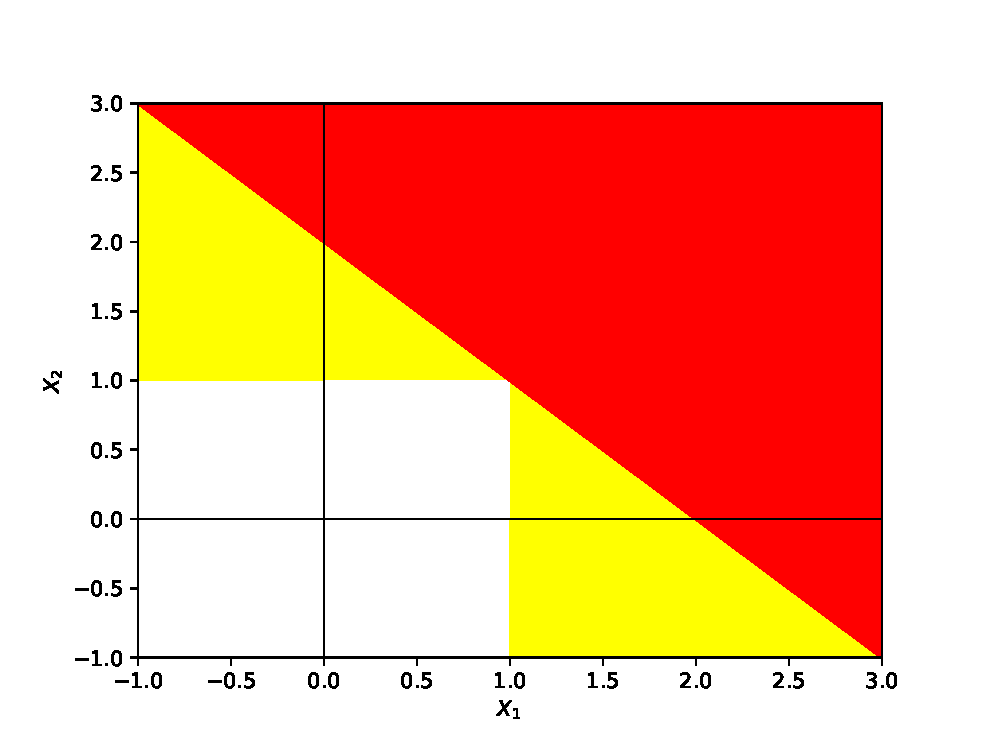
\includegraphics[width=\textwidth]{plot1.eps}
    \begin{align*}
        \P{\max(X_1,X_2)>1 \cup X>1}=\P{\max(X_1,X_2)>1} = 1-\Phi(1/\sqrt{2})^2
    \end{align*}
    $\set{\max(X_1,X_2)>1 \cup \min(X_1,X_2)>0}$ can be visualized by the following plot.
    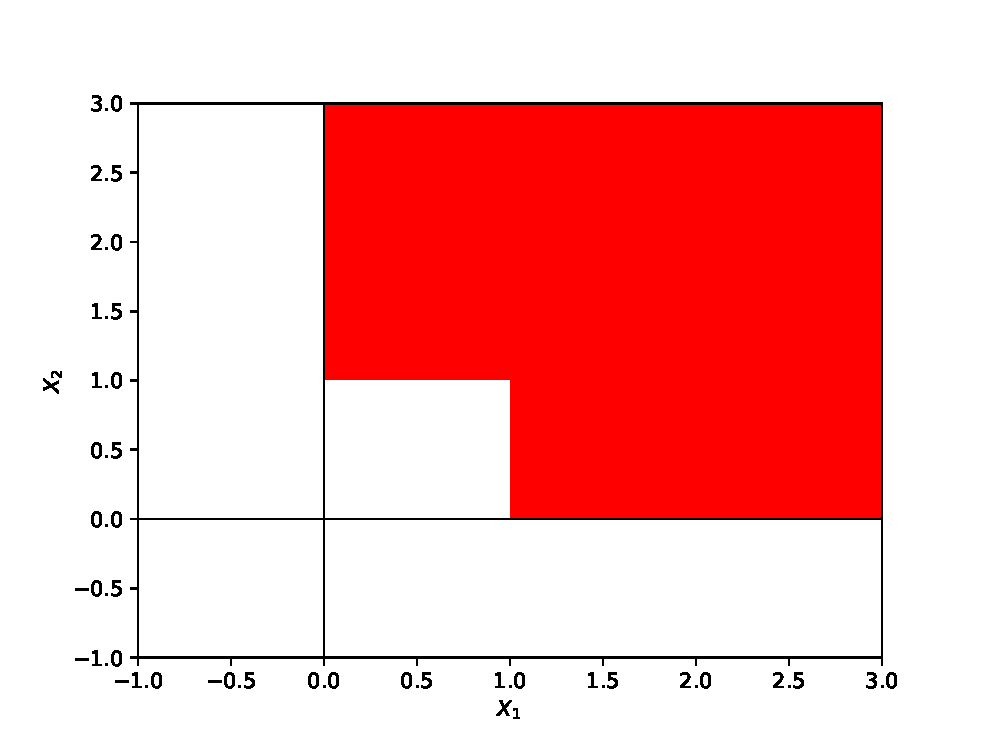
\includegraphics[width=\textwidth]{plot2.eps}
    \begin{align*}
        \P{A}
        &= \P{\max(X_1,X_2)>1 \cup \min(X_1,X_2)>0} \\
        &= \P{X_1>0,X_2>0}-\P{0<X_1<1,0<X_2<1} \\
        &= \P{X_1>0}\P{X_2>0}-\P{0<X_1<1}\P{0<X_2<1} \\
        &= (1-\P{X_1\leq 0})(1-\P{X_2\leq 0})-(\P{X_1\leq 1}-\P{X_1\leq 0})(\P{X_2\leq 1}-\P{X_2\leq 0}) \\
        &= (1-\Phi(0))^2-(\Phi(1/\sqrt{2})-\Phi(0))^2
    \end{align*}
\end{solution}

\begin{problem}
    {Group 2}
    Let $X$ and $Y$ be continues random variables with joint PDF
    \[
    f(x,y) = {
        \begin{cases}
            2 & 0\leq y\leq x\leq 1,\\
            0 & \text{otherwise.}
        \end{cases}
    }
    \]
    \begin{enumerate}
        \item What are $\E{X}$ and $\Var(X)$?
        \item What are $\E{Y}$ and $\Var(Y)$?
        \item What are $\Cov(X,Y)$ and $\Corr(X,Y)$?
        \item What are $\E{X+Y}$ and $\Var(X+Y)$?
    \end{enumerate}
\end{problem}

\begin{solution}
    {Solution}
    \begin{align*}
        \E{X}
        &= \int_{0}^{1}\int_{y}^{1}x\cdot 2\diff x \diff y \\
        &= \int_{0}^{1}1-y^2\diff y \\
        &= \frac{2}{3} \\
        \E{X^2}
        &= \int_{0}^{1}\int_{y}^{1}x^2\cdot 2\diff x \diff y \\
        &= \int_{0}^{1}\frac{2}{3}(1-y^3)\diff y \\
        &= \frac{1}{2} \\
        \Var(X)
        &= \E{X^2}-\E{X}^2 \\
        &= \frac{1}{2}-\frac{4}{9} \\
        &= \frac{1}{18} \\
        \E{Y}
        &= \int_{0}^{1}\int_{0}^{x}y\cdot 2\diff y \diff x \\
        &= \int_{0}^{1}x^2\diff x \\
        &= \frac{1}{3} \\
        \E{Y^2}
        &= \int_{0}^{1}\int_{0}^{x}y^2\cdot 2\diff y \diff x \\
        &= \int_{0}^{1}\frac{2}{3}x^3\diff x \\
        &= \frac{1}{6} \\
        \Var(Y)
        &= \E{Y^2}-\E{Y}^2 \\
        &= \frac{1}{6}-\frac{1}{9} \\
        &= \frac{1}{18} \\
        \E{XY}
        &= \int_{0}^{1}\int_{0}^{x}xy\cdot 2\diff y \diff x \\
        &= \int_{0}^{1}x^3\diff x \\
        &= \frac{1}{4} \\
        \Cov(X,Y)
        &= \E{XY}-\E{X}\E{Y} \\
        &= \frac{1}{4}-\frac{2}{9} \\
        &= \frac{1}{36} \\
        \Corr(X,Y)
        &= \frac{\Cov(X,Y)}{\sqrt{\Var(X)\Var(Y)}} \\
        &= \frac{1}{2} \\
        \E{X+Y}
        &= \E{X}+\E{Y} \\
        &= 1 \\
        \Var(X+Y)
        &= \Var(X)+\Var(Y)+2\Cov(X,Y) \\
        &= \frac{1}{18}+\frac{1}{18}+2\frac{1}{36} \\
        &= \frac{1}{6}
    \end{align*}
\end{solution}

\begin{problem}
    {Group 3}
    A company receives shipments from two factories. Depending on the size of the order, a shipment can be in
    \begin{enumerate}
        \item 1 box for a small order,
        \item 2 boxes for a medium order,
        \item 3 boxes for a large order.
    \end{enumerate}
    The company has two different suppliers. Factory Q is 60 miles from the company. Factory R is 180 miles from the company. An experiment consists of monitoring a shipment and observing B, the number of boxes, and M, the number of miles the shipment travels. The following probability model describes the experiment:
    \begin{table}[H]
        \centering
        \begin{tabular}{|l|l|l|}
        \hline
                     & Factory Q & Factory R \\ \hline
        small order  & 0.3       & 0.2       \\ \hline
        medium order & 0.1       & 0.2       \\ \hline
        large order  & 0.1       & 0.1       \\ \hline
        \end{tabular}
    \end{table}
    \begin{enumerate}
        \item Find $P_{B,M}(b,m)$, the joint PMF of the number of boxes and the distance.
        \item What is $\E{B}$, the expected number of boxes?
        \item Are $B$ and $M$ independent?
    \end{enumerate}
\end{problem}

\begin{solution}
    {Solution}
    \[
    P_{B,M}(b,m)={
        \begin{cases}
            0.3 & b=1, m=60\\
            0.2 & b=1, m=180\\
            0.1 & b=2, m=60\\
            0.2 & b=2, m=180\\
            0.1 & b=3, m=60\\
            0.1 & b=3, m=180\\
            0 & \text{otherwise}
        \end{cases}
    }
    \]
    \[
    \E{B}= 1\cdot 0.3+1\cdot 0.2+2\cdot 0.1+2\cdot 0.2+3\cdot 0.1+3\cdot 0.1=1.7
    \]
    No, $B$ and $M$ are not independent. Because $P_{B,M}(1,60)=0.3\neq 0.25=0.5\cdot 0.5=P_B(1)P_M(60)$.
\end{solution}

\begin{problem}
    {Group 4}
    Random Variables $N$ and $K$ have the joint PMF
    \[
    P_{N,K}(n,k)={
        \begin{cases}
            \frac{(1-p)^{n-1}p}{n} & k=1,2,\ldots,n; n=1,2,\ldots\\
            0 & \text{otherwise.}
        \end{cases}
    }
    \]
    Find $P_N(n)$, $\E{N}$, $\Var(N)$, $\E{N^2}$, $\E{K}$, $\Var(K)$, $\E{N+K}$, $r_{N,K}$, $\Cov(N,K)$.
    \begin{solution}
        {Hint:}
        Please solve the first four and leave the rest for me.
    \end{solution}
\end{problem}

\begin{solution}
    {Solution}
    \[
    P_N(n)={
        \begin{cases}
            \sum_{k=1}^{n}\frac{(1-p)^{n-1}p}{n}=n\cdot\frac{(1-p)^{n-1}p}{n}=(1-p)^{n-1}p & n=1,2,\ldots\\
            0 & \text{otherwise.}
        \end{cases}
    }
    \]
    \[
    \E{N} = \frac{1}{p} \qquad \Var[N] = \frac{1-p}{p^2} \qquad \E{N^2} = \Var[N] + \E{N}^2 = \frac{2-p}{p^2}
    \]
    \[
    \E{K} = \sum_{n=1}^{\infty}\sum_{k=1}^{n}k\cdot\frac{(1-p)^{n-1}p}{n} = \sum_{n=1}^{\infty}\frac{(1-p)^{n-1}p}{n}\sum_{k=1}^{n}k = \sum_{n=1}^{\infty}\frac{(1-p)^{n-1}p}{n}\frac{n(n+1)}{2}
    \]
    Since $\sum_{n=1}^{\infty}(1-p)^{n-1}p=1$
    \[
        \E{K} = \E{\frac{N+1}{2}} = \frac{\E{N}+1}{2} = \frac{1}{2p}+\frac{1}{2}
    \]
    Following the same logic,
    \[
    \E{K^2} = \E{\frac{(N+1)(2N+1)}{6}}=\frac{2\E{N^2}+3\E{N}+1}{6}= \frac{2-p}{3p^2}+\frac{1}{2p}+\frac{1}{6}
    \]
    \[
    \Var[K] = \E{K^2}-\E{K}^2 = \frac{2-p}{3p^2}+\frac{1}{2p}+\frac{1}{6}-\left(\frac{1}{2p}+\frac{1}{2}\right)^2
    \]
    \begin{align*}
        r_{N,K}
        &= \E{NK} \\
        &= \E{\sum_{n=1}^{\infty}\sum_{k=1}^{n}nk\cdot\frac{(1-p)^{n-1}p}{n}} \\
        &= \E{\sum_{n=1}^{\infty}(1-p)^{n-1}p\sum_{k=1}^{n}k} \\
        &= \E{\sum_{n=1}^{\infty}(1-p)^{n-1}p\frac{n(n+1)}{2}} \\
        &= \E{\frac{N(N+1)}{2}} \\
        &= \frac{1}{2}\E{N^2}+\frac{1}{2}\E{N} \\
        &= \frac{2-p}{2p^2}+\frac{1}{2p} = \frac{1}{p^2}
    \end{align*}
    \[
    \Cov(N,K) = r_{N,K}-\E{N}\E{K} = \frac{1}{p^2}-\frac{1}{p}\frac{1}{2p}-\frac{1}{2p} = \frac{1}{2p^2}-\frac{1}{2p}
    \]
\end{solution}

\begin{problem}
    {Group 5}
    $X$ and $Y$ are random variables such that $X$ has expected value $\mu_X = 0$ and standard deviation $\sigma_X = 3$ while $Y$ has expected value $\mu_Y = 1$ and standard deviation $\sigma_Y = 4$. In addition, $X$ and $Y$ have covariance $\Cov[X, Y] = -3$. Find the expected value and variance of $W = 2X+2Y$.
\end{problem}

\begin{solution}
    {Solution}
    \[
        \E{W} = \E{2X+2Y} = 2\E{X}+2\E{Y} = 2\cdot 0+2\cdot 1 = 2
    \]
    \[
        \Var(W) = \Var(2X+2Y) = 4\Var(X)+4\Var(Y)+8\Cov(X,Y) = 4\cdot 3^2+4\cdot 4^2+8\cdot (-3) = 76
    \]
\end{solution}
% \fi
% \iffalse
%%%% HW 11
\begin{problem}
    {Group 1}
    The expectation of $\Geomv(p)$ can be proved by conditional expectation as follows:
    \begin{proof}
        For $X\sim\Geomv(p)$,
        \begin{align*}
            \E{X}
            &= \condE{X}{X=1}\P{X=1}+\condE{X}{X>1}\P{X>1}\\
            &= \E{X=1}\cdot p + \E{X+1}(1-p)\\
            \Rightarrow
            \E{X} &= \frac{1}{p}.
        \end{align*}
    \end{proof}
    Following the same logic, derive the Variance of $\Geomv(p)$.
\end{problem}

\begin{solution}
    {Solution}
    \begin{align*}
        \E{X^2}
        &= \condE{X^2}{X=1}\P{X=1}+\condE{X^2}{X>1}\P{X>1}\\
        &= \E{X=1^2}\cdot p + \E{(X+1)^2}(1-p)\\
        &= 1\cdot p + \E{X^2+2X+1}(1-p)\\
        &= p + \E{X^2}(1-p)+2\E{X}(1-p)+1(1-p)\\
        \Rightarrow
        \E{X^2}
        &= \frac{2}{p^2}-\frac{1}{p}\\
        \Var[X]
        &= \E{X^2}-\E{X}^2 \\
        &= \frac{2}{p^2}-\frac{1}{p}-\frac{1}{p^2} \\
        &= \frac{1-p}{p^2}.
    \end{align*}
\end{solution}

\begin{problem}
    {Group 2}
    Let $Y_1$ denote the weight (in tons) of a bulk item stocked by a supplier at the beginning of a week and suppose that $Y_1$ has a uniform distribution over the interval $0 \leq y_1 \leq 1$. Let $Y_2$ denote the amount (by weight) of this item sold by the supplier during the week and suppose that $Y_2$ has a uniform distribution over the interval $0 \leq y_2 \leq y_1$, where $y_1$ is a specific value of $Y_1$.
    \begin{enumerate}
        \item Find the joint density function for $Y_1$ and $Y_2$.
        \item If the supplier stocks a half-ton of the item, what is the probability that she sells more than a quarter-ton?
        \item If it is known that the supplier sold a quarter-ton of the item, what is the probability that she had stocked more than a half-ton?
    \end{enumerate}
\end{problem}

\begin{solution}
    {Solution}
    \begin{enumerate}
        \item
        \begin{align*}
            f_{Y_1,Y_2}(y_1,y_2)
            &= f_{Y_2\mid Y_1}(y_2\mid y_1)f_{Y_1}(y_1) \\
            &= \frac{1}{y_1}\cdot 1 \\
            f_{Y_1,Y_2}(y_1,y_2)
            &={
            \begin{cases}
                \frac{1}{y_1} & 0\leq y_2\leq y_1\leq 1\\
                0 & \text{otherwise.}
            \end{cases}
        }
        \end{align*}
        \item
        \begin{align*}
            f_{Y_2\mid Y_1}(y_2\mid y_1)
            &= \frac{f_{Y_1,Y_2}(y_1,y_2)}{f_{Y_1}(y_1)} \\
            &= \frac{\frac{1}{y_1}}{\int_{0}^{y_1}\frac{1}{y_1}\diff y_2} \\
            &= \frac{\frac{1}{y_1}}{1}\\
            &= \frac{1}{y_1} \\
            \condP{Y_2>0.25}{Y_1=0.5}
            &= \int_{0.25}^{0.5}\frac{1}{0.5}\diff y_2 \\
            &= 0.5
        \end{align*}
        \item
        \begin{align*}
            f_{Y_1\mid Y_2}(y_1\mid y_2)
            &= \frac{f_{Y_1,Y_2}(y_1,y_2)}{f_{Y_2}(y_2)} \\
            &= \frac{\frac{1}{y_1}}{\int_{y_2}^{1}\frac{1}{y_1}\diff y_1} \\
            &= \frac{\frac{1}{y_1}}{-\ln y_2} \\
            &= \frac{1}{y_1(-\ln y_2)} \\
            \P{Y_1>0.5\mid Y_2=0.25}
            &= \int_{0.5}^{1}\frac{1}{y_1(-\ln 0.25)}\diff y_1 \\
            &= \frac{\ln 2}{2\ln 2} \\
            &= 0.5
        \end{align*}
    \end{enumerate}
\end{solution}

\begin{problem}
    {Group 3}
    A quality control plan calls for randomly selecting three items from the daily production (assumed large) of a certain machine and observing the number of defectives. However, the proportion p of defectives produced by the machine varies from day to day and is assumed to have a uniform distribution on the interval (0, 1). For a randomly chosen day, find the unconditional probability that exactly two defectives are observed in the sample.
\end{problem}

\begin{solution}
    {Solution}
    \begin{align*}
        \condP{Y=y}{p}
        &= \binom{3}{y}p^y(1-p)^{3-y} \qquad y=0,1,2,3 \\
        \P{Y=2}
        &= \int_{0}^{1} \P{Y=2, p}\diff p \\
        &= \int_{0}^{1}\condP{Y=2}{p}f_P(p)\diff p \\
        &= \int_{0}^{1}\binom{3}{2}p^2(1-p)^{3-2}\cdot 1\diff p \\
        &= \int_{0}^{1}3p^2(1-p)\diff p \\
        &= \int_{0}^{1}(3p^2-3p^3)\diff p \\
        &= \left[p^3-\frac{3}{4}p^4\right]_{0}^{1} \\
        &= 1-\frac{3}{4} \\
        &= \frac{1}{4}
    \end{align*}
\end{solution}

\begin{problem}
    {Group 4}
    Suppose that the probability that a head appears when a coin is tossed is $p$ and the probability that a tail occurs is $q = 1 - p$. Person A tosses the coin until the first head appears and stops. Person B does likewise. The results obtained by persons A and B are assumed to be independent. What is the probability that A and B stop on exactly the same number toss? Explain how you think. The calculation is not mandatory.
\end{problem}

\begin{solution}
    {Solution}
    \begin{align*}
        &\P{A=1,B=1}+\P{A=2,B=2}+\P{A=3,B=3}+\ldots \\
        = &\P{A=1}\P{B=1}+\P{A=2}\P{B=2}+\P{A=3}\P{B=3}+\ldots \\
        = &\sum_{i=1}^{\infty}\P{A=i}\P{B=i} \\
        = &\sum_{i=1}^{\infty}pq^{i-1}pq^{i-1} \\
        = &p^2\sum_{i=1}^{\infty}(q^2)^{i-1} \\
        = &\frac{p^2}{1-q^2}
    \end{align*}
\end{solution}

\begin{problem}
    {Group 5}
    Let $Y_1$ and $Y_2$ be independent exponentially distributed random variables, each with mean $1$. Find $P( Y_1 > Y_2 \mid Y_1 < 2Y_2)$ and $P( Y_1 < 2Y_2 \mid Y_1 > Y_2)$.
    \begin{solution}
        {Hint:}
        \begin{enumerate}
            \item Find the joint probability of $Y_1$ and $Y_2$.
            \item Determine the range of $Y_1$ and $Y_2$ that satisfies the condition.
            \item Use the definition of conditional probability.
            \item Surprisingly, $P( Y_1 < 2Y_2 \mid Y_1 > Y_2)$ is much easier to calculate than $P( Y_1 = 2Y_2 \mid Y_1 > Y_2)$.
        \end{enumerate}
    \end{solution}
\end{problem}

\begin{solution}
    {Solution}
    \begin{align*}
        f_{Y_1,Y_2}(y_1,y_2)
        &= f_{Y_1}(y_1)f_{Y_2}(y_2) \\
        &= e^{-y_1}e^{-y_2} \\
        &= e^{-(y_1+y_2)} \\
        \P{Y_1>Y_2\mid Y_1<2Y_2}
        &= \frac{\P{Y_1>Y_2,Y_1<2Y_2}}{\P{Y_1<2Y_2}} \\
        &= \frac{\int_{0}^{\infty}\int_{y_2}^{2y_2}e^{-(y_1+y_2)}\diff y_1\diff y_2}{\int_{0}^{\infty}\int_{0}^{2y_2}e^{-(y_1+y_2)}\diff y_1\diff y_2} \\
        &= \frac{\frac{1}{6}}{\frac{2}{3}} \\
        &= \frac{1}{4} \\
        \P{Y_1<2Y_2\mid Y_1>Y_2}
        &= \frac{\P{Y_1<2Y_2,Y_1>Y_2}}{\P{Y_1>Y_2}} \\
        &= \frac{\int_{0}^{\infty}\int_{y_2}^{2y_2}e^{-(y_1+y_2)}\diff y_1\diff y_2}{\int_{0}^{\infty}\int_{y_2}^{\infty}e^{-(y_1+y_2)}\diff y_1\diff y_2} \\
        &= \frac{\frac{1}{6}}{\frac{1}{2}} \\
        &= \frac{1}{3}
    \end{align*}
\end{solution}
% \fi
% \iffalse
%%%% HW 12
\begin{problem}
    {Group 1}
    A coin that has probability of heads equal to $p$ is tossed successively and independently until a head comes twice in a row or a tail comes twice in a row. Find the expected value of the number of tosses in terms of $p$ and $q=1-p$.
    \begin{solution}
        {Hint:}
        The Law of Total Expectation is useful.
    \end{solution}
\end{problem}

\begin{solution}
    {Solution}
    With the law of total probability, we can partition the event $X$ based on the first (starting from $0$) toss,
    \[
        \P{X}=\P{X\mid H_0}\P{H_0}+\P{X\mid T_0}\P{T_0}.
    \]
    Similarly, each partition of the first toss can be partitioned based on the second toss,
    \begin{align*}
        \P{X\mid H_0} &= \P{X\mid H_0\cap H_1}\P{H_1}+\P{X\mid H_0\cap T_1}\P{T_1}, \\
        \P{X\mid T_0} &= \P{X\mid T_0\cap H_1}\P{H_1}+\P{X\mid T_0\cap T_1}\P{T_1}.
    \end{align*}
    Apply expectation to both sides,
    \begin{align*}
        \E{X} &= \E{X\mid H_0}\P{H_0}+\E{X\mid T_0}\P{T_0}, \\
        \E{X\mid H_0} &= \E{X\mid H_0\cap H_1}\P{H_1}+\E{X\mid H_0\cap T_1}\P{T_1}, \\
        \E{X\mid T_0} &= \E{X\mid T_0\cap H_1}\P{H_1}+\E{X\mid T_0\cap T_1}\P{T_1}.
    \end{align*}
    Because the game will end with two heads/tails in a row or start counting over, we have
    \[
    \E{X\mid H_0H_1}= \E{X\mid T_0T_1}=2, \qquad \E{X\mid H_0T_1} = 1+\E{X\mid T_0}, \qquad \E{X\mid T_0H_1} = 1+\E{X\mid H_0}.
    \]
    \begin{align*}
        \E{X\mid H_0} &= 2p+(1+\E{X\mid T_0})q, \\
        \E{X\mid T_0} &= (1+\E{X\mid H_0})p+2q, \\
        \Rightarrow
        \E{X\mid H_0} &= \frac{2+q^2}{1-pq}, \\
        \E{X\mid T_0} &= \frac{2+p^2}{1-pq}, \\
        \Rightarrow
        \E{X} &= \frac{2+q^2}{1-pq}p+\frac{2+p^2}{1-pq}q \\
        &= \frac{2p+q^2p+2q+p^2q}{1-pq} \\
        &= \frac{2(p+q)+(q+p)pq}{1-pq} \\
        &= \frac{2+pq}{1-pq}.
    \end{align*}
\end{solution}

\begin{problem}
    {Group 2}
    $X$ and $Y$ are independent identical discrete uniform $(1, 10)$ random variables. Find the conditional PMF $P_{X,Y \mid A}(x, y)$. Let $A$ denote the event that
    \begin{enumerate}
        \item $\min(X, Y) > 5$.
        \item $\max(X, Y) \leq 5$.
    \end{enumerate}
    \begin{solution}
        {Hint:}
        For discrete random variables, you can always list all the possible values and their corresponding probabilities.
    \end{solution}
\end{problem}

\begin{solution}
    {Solution}
    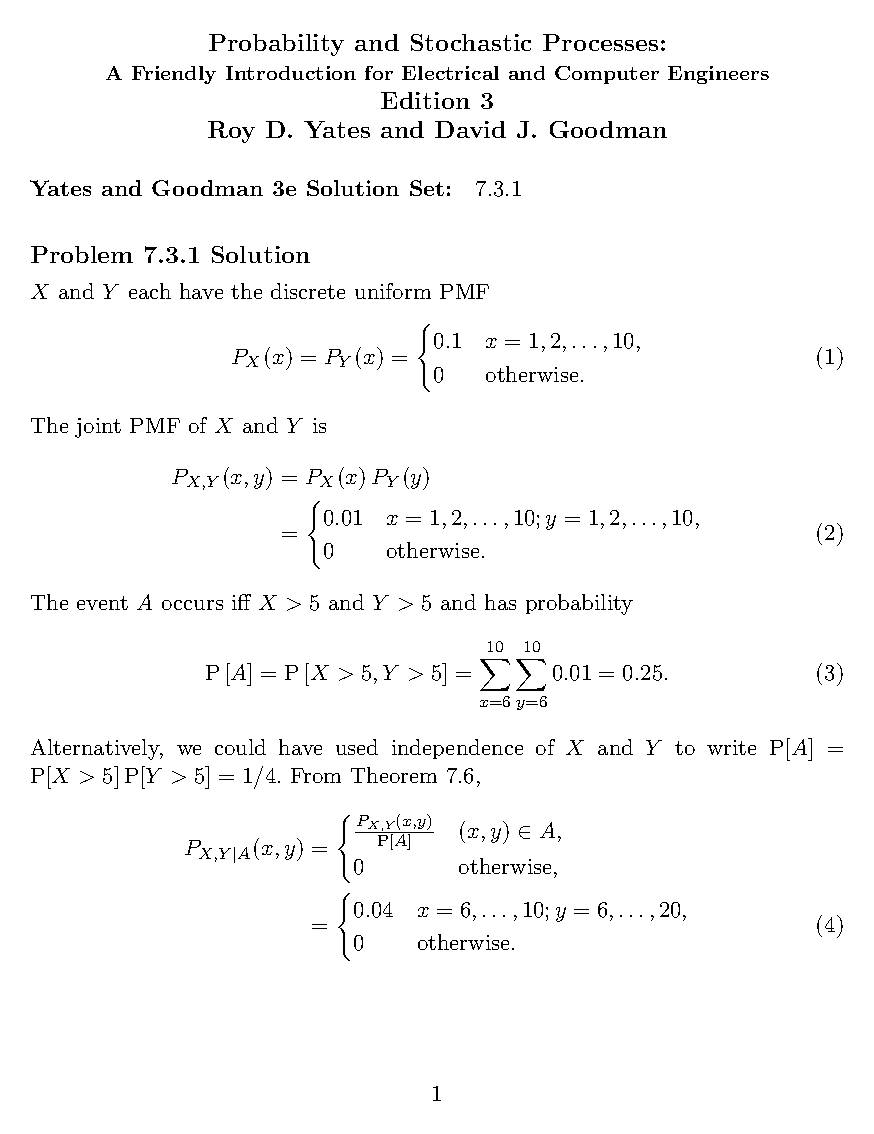
\includegraphics[width=0.6\textwidth, center]{winlab-ms6Z3OUCPY-s.pdf}
    And the same for the second case.
\end{solution}

\begin{problem}
    {Group 3}
    A supermarket has two customers waiting to pay for their purchases at counter I and one customer waiting to pay at counter II. Let $Y_1$ and $Y_2$ denote the numbers of customers who spend more than \$50 on groceries at the respective counters. Suppose that $Y_1$ and $Y_2$ are independent binomial random variables, with the probability that a customer at counter I will spend more than \$50 equal to $.2$ and the probability that a customer at counter II will spend more than \$50 equal to $.3$. Find the
    \begin{enumerate}
        \item joint probability distribution for $Y_1$ and $Y_2$.
        \item probability that not more than one of the three customers will spend more than \$50.
    \end{enumerate}
\end{problem}

\begin{solution}
    {Solution}
    \begin{align*}
        P_{Y_1}(y_1) &= \binom{2}{y_1}0.2^{y_1}0.8^{2-y_1}, \qquad y_1=0,1,2 \\
        P_{Y_2}(y_2) &= \binom{1}{y_2}0.3^{y_2}0.7^{1-y_2}, \qquad y_2=0,1 \\
        P_{Y_1,Y_2}(y_1,y_2) &= P_{Y_1}(y_1)P_{Y_2}(y_2) \\
        &= \binom{2}{y_1}0.2^{y_1}0.8^{2-y_1}\binom{1}{y_2}0.3^{y_2}0.7^{1-y_2}, \qquad y_1=0,1,2 \quad y_2=0,1 \\
        \P{Y_1+Y_2\leq 1} &= \P{0,0} + \P{1,0} + \P{0,1} \\
        &= 0.8^2\cdot 0.7 + 2\cdot 0.2\cdot 0.8\cdot 0.7 + 0.8^2\cdot 0.3 \\
        &= 0.864
    \end{align*}
\end{solution}

\begin{problem}
    {Group 4}
    The length of life $Y$ for fuses of a certain type is modeled by the exponential distribution, with rate $\lambda=1/3$ (The measurements are in hundreds of hours.).
    \begin{enumerate}[(a)]
        \item If two such fuses have independent lengths of life $Y_1$ and $Y_2$, find the joint probability density function for $Y_1$ and $Y_2$.\label{item:4a}
        \item One fuse in \cref{item:4a} is in a primary system, and the other is in a backup system that comes into use only if the primary system fails. The total effective length of life of the two fuses is then $Y_1 + Y_2$. Find $\P{Y_1 + Y_2 \leq 1}$.
    \end{enumerate}
\end{problem}

\begin{solution}
    {Solution}
    \begin{align*}
        f_{Y_1,Y_2}(y_1,y_2)&= f_{Y_1}(y_1)f_{Y_2}(y_2) \\
        &= \frac{1}{3}e^{-\frac{1}{3}y_1}\frac{1}{3}e^{-\frac{1}{3}y_2} \\
        &= \frac{1}{9}e^{-\frac{1}{3}(y_1+y_2)} \\
        \P{Y_1+Y_2\leq 1} &= \int_{0}^{1}\int_{0}^{1-y_1}\frac{1}{9}e^{-\frac{1}{3}(y_1+y_2)}\diff y_2\diff y_1 \\
        &= 1-\frac{4}{3}e^{-\frac{1}{3}}
    \end{align*}
\end{solution}

\begin{problem}
    {Group 5}
    A bus arrives at a bus stop at a uniformly distributed time over the interval $0$ to $1$ hour. A passenger also arrives at the bus stop at a uniformly distributed time over the interval $0$ to $1$ hour. Assume that the arrival times of the bus and passenger are independent of one another and that the passenger will wait for up to $1/4$ hour for the bus to arrive. What is the probability that the passenger will catch the bus?
    \begin{solution}
        {Hint:}
        \begin{enumerate}
            \item Let $Y_1$ denote the bus arrival time and $Y_2$ the passenger arrival time.
            \item Determine the joint density of $Y_1$ and $Y_2$.
            \item Find $\P{Y_2 \leq Y_1 \leq Y_2 + 1/4}$.
        \end{enumerate}
    \end{solution}
\end{problem}

\begin{solution}
    {Solution}
    % The region of \[Y_2 \leq Y_1 \leq Y_2 + 1/4\]
    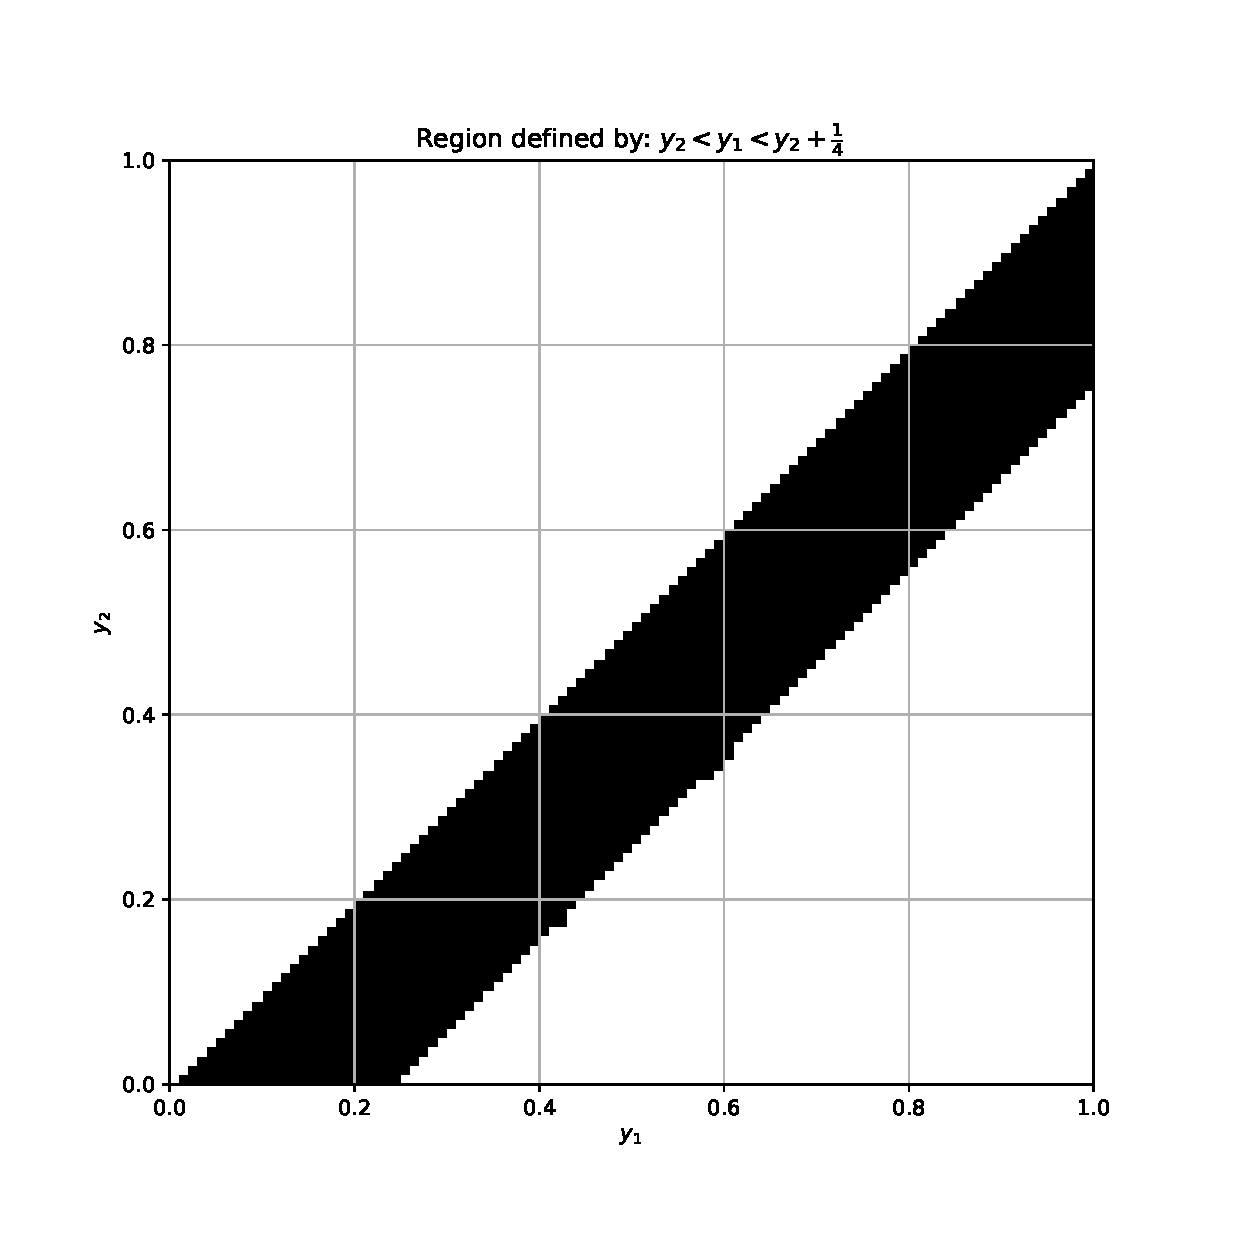
\includegraphics[width=0.9\textwidth, center]{plot3.eps}

    The black area is
    \[
    1\cdot1\cdot\frac{1}{2}-\frac{3}{4}\cdot\frac{3}{4}\cdot\frac{1}{2}=\frac{7}{32}.
    \]
\end{solution}
% \fi
% \iffalse
%%%% HW 13
\begin{problem}
    {Group 1}
    Two telephone calls uniformly come into a switchboard at random times in a fixed one-hour period. Assume that the calls are made independently of one another. What is the probability that the calls are made
    \begin{enumerate}
        \item in the first half hour?
        \item within five minutes of each other?
    \end{enumerate}
\end{problem}

\begin{solution}
    {Solution}
    Let $X_1$ and $X_2$ be the arrival times of the two calls. Then $X_1$ and $X_2$ are independent and uniformly distributed over the interval $[0,1]$. The joint density of $X_1$ and $X_2$ is
    \[
        f_{X_1,X_2}(x_1,x_2) = {
            \begin{cases}
                1 & 0\leq x_1\leq 1, 0\leq x_2\leq 1 \\
                0 & \text{otherwise.}
            \end{cases}
        }
    \]
    \begin{align*}
        \P{X_1,X_2\leq 0.5}
        &= \int_{0}^{0.5}\int_{0}^{0.5}1\diff x_1\diff x_2 \\
        &= \frac{1}{4}
    \end{align*}
    The area of the region where $|X_1-X_2|\leq 1/12$ is

    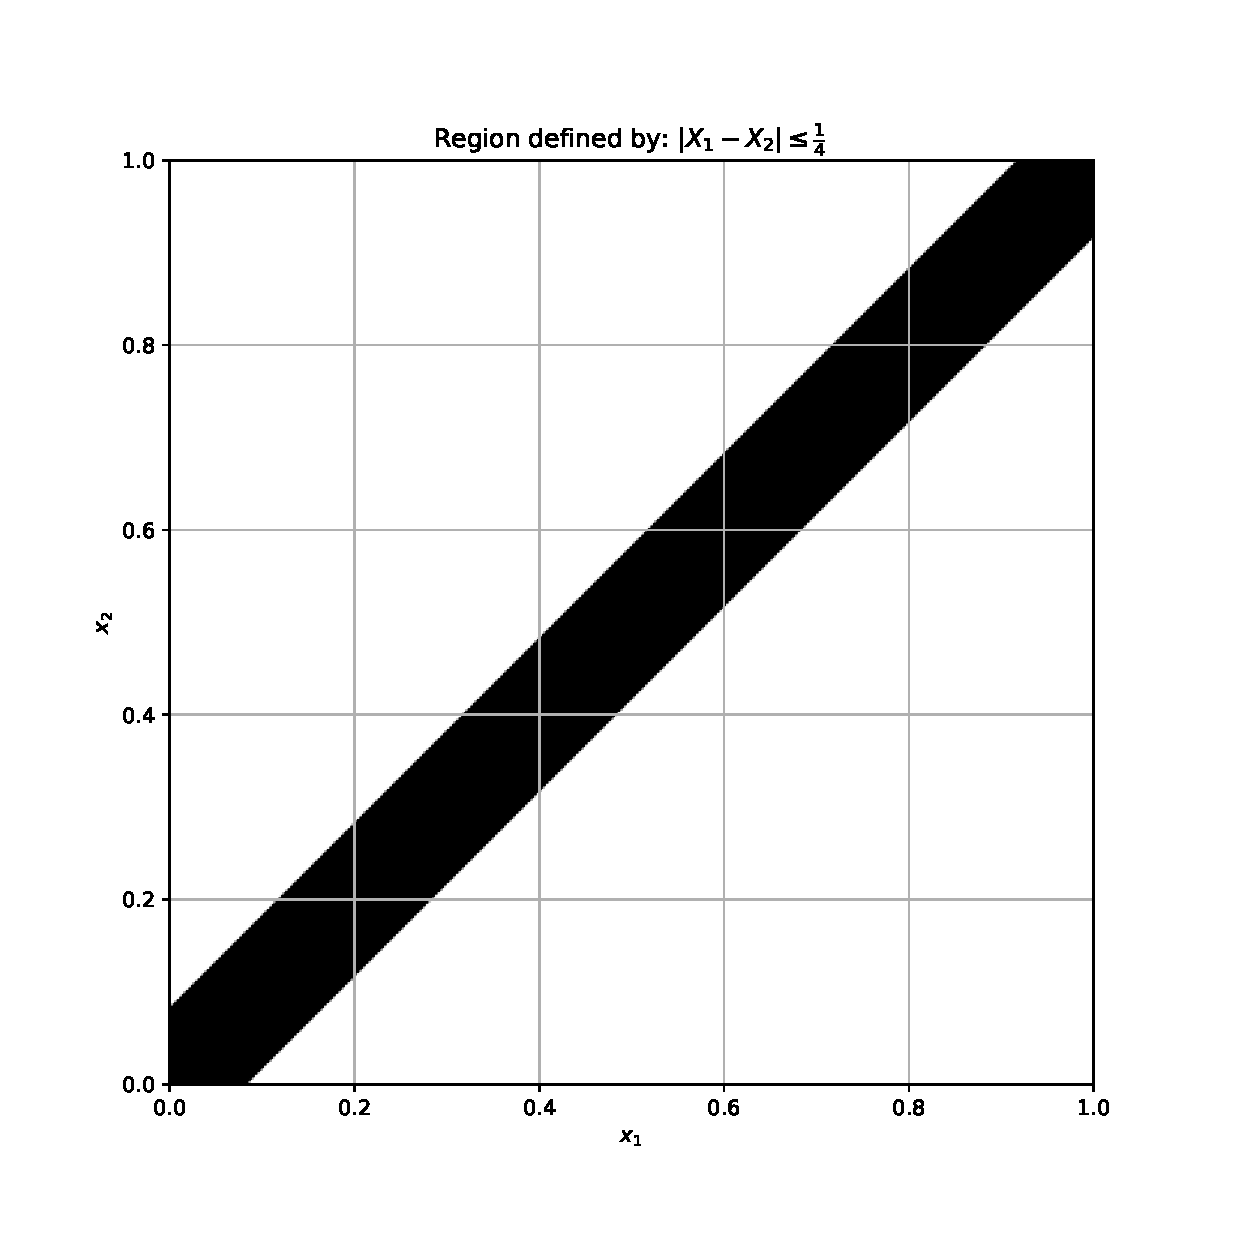
\includegraphics[width=\textwidth, center]{plot4.eps}
    and the $\P{|X_1-X_2|\leq 1/12}=1-\frac{1}{2}(\frac{11}{12})^2\times2=\frac{23}{144}$.
\end{solution}

\begin{problem}
    {Group 2}
    A process for producing an industrial chemical yields a product containing two types of impurities. For a specified sample from this process, let $Y_1$ denote the proportion of impurities in the sample and let $Y_2$ denote the proportion of type I impurities among all impurities found. Suppose that the joint distribution of $Y_1$ and $Y_2$ can be modeled by the following probability density function:
    \[
    f_{Y_1,Y_2}(y_1,y_2)={
        \begin{cases}
            2(1-y_1) & 0\leq y_1\leq1, 0\leq y_2\leq 1\\
            0 & \text{otherwise.}
        \end{cases}
    }
    \]
    Find the expected value of the proportion of type I impurities in the sample.
\end{problem}

\begin{solution}
    {Solution}
    \begin{align*}
        \E{Y_1Y_2}
        &= \int_{0}^{1}\int_{0}^{1}y_1y_2\cdot 2(1-y_1)\diff y_1\diff y_2 \\
        &= \int_{0}^{1}\int_{0}^{1}2y_1y_2-2y_1^2y_2\diff y_1\diff y_2 \\
        &= \int_{0}^{1}y_2-\frac{2}{3}y_2\diff y_2 \\
        &= \frac{1}{2}-\frac{1}{3} \\
        &= \frac{1}{6}
    \end{align*}
\end{solution}

\begin{problem}
    {Group 3}
    Let the discrete random variables $Y_1$ and $Y_2$ have the joint probability function $P_{Y_1,Y_2}(y_1, y_2) = 1/3$, for $(y_1, y_2) = (-1, 0), (0, 1), (1, 0)$. Find $\Cov(Y_1, Y_2)$. Notice that $Y_1$ and $Y_2$ are dependent. (Why?) This is another example of uncorrelated random variables that are not independent.
\end{problem}

\begin{solution}
    {Solution}
    \begin{align*}
        P_{Y_1}(y_1) &= {
            \begin{cases}
                1/3 & y_1=-1, 0, 1 \\
                0 & \text{otherwise.}
            \end{cases}
        }\\
        P_{Y_2}(y_2) &= {
            \begin{cases}
                2/3 & y_2=0 \\
                1/3 & y_2=1 \\
                0 & \text{otherwise.}
            \end{cases}
        }\\
        \E{Y_1}
        &= -1\cdot\frac{1}{3}+0\cdot\frac{1}{3}+1\cdot\frac{1}{3} \\
        &= 0 \\
        \E{Y_2}
        &= 0\cdot\frac{2}{3}+1\cdot\frac{1}{3} \\
        &= \frac{1}{3} \\
        \E{Y_1Y_2}
        &= -1\cdot 0\cdot\frac{1}{3}+0\cdot 1\cdot\frac{1}{3}+1\cdot 0\cdot\frac{1}{3} \\
        &= 0 \\
        \Cov(Y_1,Y_2)
        &= \E{Y_1Y_2}-\E{Y_1}\E{Y_2} \\
        &= 0-0\cdot\frac{1}{3} \\
        &= 0
    \end{align*}
\end{solution}

\begin{problem}
    {Group 4}
    Suppose that $Y_1$ and $Y_2$ have correlation coefficient $\rho = .2$. What is the value of the correlation coefficient between
    \begin{enumerate}
        \item $1 + 2Y_1$ and $3 + 4Y_2$?
        \item $1 + 2Y_1$ and $3 - 4Y_2$?
        \item $1 - 2Y_1$ and $3 - 4Y_2$?
    \end{enumerate}
    \begin{solution}
        {Hint:}
        Use the variance of derived random variable and the definition of correlation coefficient.
    \end{solution}
\end{problem}

\begin{solution}
    {Solution}
    \begin{align*}
        \rho_{1+2Y_1,3+4Y_2} &= \frac{\Cov(1+2Y_1,3+4Y_2)}{\sqrt{\Var(1+2Y_1)}\sqrt{\Var(3+4Y_2)}} \\
        &= \frac{\Cov(2Y_1,4Y_2)}{\sqrt{\Var(2Y_1)}\sqrt{\Var(4Y_2)}} \\
        &= \frac{2\cdot 4\Cov(Y_1,Y_2)}{2\cdot 4\sqrt{\Var(Y_1)}\sqrt{\Var(Y_2)}} \\
        &= \frac{\Cov(Y_1,Y_2)}{\sqrt{\Var(Y_1)}\sqrt{\Var(Y_2)}} \\
        &= \rho = 0.2 \\
        \rho_{1+2Y_1,3-4Y_2} &= \frac{\Cov(1+2Y_1,3-4Y_2)}{\sqrt{\Var(1+2Y_1)}\sqrt{\Var(3-4Y_2)}} \\
        &= \frac{\Cov(2Y_1,-4Y_2)}{\sqrt{\Var(2Y_1)}\sqrt{\Var(-4Y_2)}} \\
        &= \frac{2\cdot (-4)\Cov(Y_1,Y_2)}{2\cdot 4\sqrt{\Var(Y_1)}\sqrt{\Var(Y_2)}} \\
        &= -\frac{\Cov(Y_1,Y_2)}{\sqrt{\Var(Y_1)}\sqrt{\Var(Y_2)}} \\
        &= -\rho = -0.2 \\
        \rho_{1-2Y_1,3-4Y_2} &= \frac{\Cov(1-2Y_1,3-4Y_2)}{\sqrt{\Var(1-2Y_1)}\sqrt{\Var(3-4Y_2)}} \\
        &= \frac{\Cov(-2Y_1,-4Y_2)}{\sqrt{\Var(-2Y_1)}\sqrt{\Var(-4Y_2)}} \\
        &= \frac{(-2)\cdot (-4)\Cov(Y_1,Y_2)}{2\cdot 4\sqrt{\Var(Y_1)}\sqrt{\Var(Y_2)}} \\
        &= \frac{\Cov(Y_1,Y_2)}{\sqrt{\Var(Y_1)}\sqrt{\Var(Y_2)}} \\
        &= \rho = 0.2
    \end{align*}
\end{solution}

\begin{problem}
    {Group 5}
    Let $Y_1$ and $Y_2$ have a joint density function given by
    \[
        f_{Y_1,Y_2} (y_1, y_2) = {
            \begin{cases}
                3y_1 & 0 \leq y_2 \leq y_1 \leq 1,\\
                0 & elsewhere.
            \end{cases}
        }
    \]
    \begin{enumerate}
        \item Find the marginal density functions of $Y_1$ and $Y_2$.
        \item Find $\condP{Y_1 \leq 3/4}{Y_2 \leq 1/2}$.
        \item Find the conditional density function of $Y_1$ given $Y_2 = y_2$.
        \item Find $\condP{Y_1 \leq 3/4}{Y_2 = 1/2}$.
    \end{enumerate}
\end{problem}

\begin{solution}
    {Solution}
    \begin{align*}
        P_{Y_1}(y_1) &= \int_{0}^{y_1}3y_1\diff y_2 \\
        &= 3y_1^2 \\
        P_{Y_2}(y_2) &= \int_{y_2}^{1}3y_1\diff y_1 \\
        &= \frac{3}{2}(1-y_2^2) \\
        \condP{Y_1\leq 3/4}{Y_2\leq 1/2}
        &= \frac{\P{Y_1\leq 3/4,Y_2\leq 1/2}}{\P{Y_2\leq 1/2}} \\
        &= \frac{\int_{0}^{1/2}\int_{y_2}^{3/4}3y_1\diff y_1\diff y_2}{\int_{0}^{1/2}\frac{3}{2}(1-y_2^2)\diff y_2} \\
        &= \frac{\frac{23}{64}}{\frac{11}{16}} \\
        &= \frac{23}{44} \\
        f_{Y_1\mid Y_2}(y_1\mid y_2)
        &= \frac{f_{Y_1,Y_2}(y_1,y_2)}{f_{Y_2}(y_2)} \\
        &= \frac{3y_1}{\frac{3}{2}(1-y_2^2)} \\
        &= \frac{2y_1}{1-y_2^2} \\
        \condP{Y_1\leq 3/4}{Y_2=1/2}
        &= \int_{0}^{3/4}\frac{2y_1}{1-(1/2)^2}\diff y_1 \\
        &= \frac{3}{4}
    \end{align*}
\end{solution}
% \fi
% \iffalse
%%%% HW 14
\begin{problem}
    {Group 1}
    Suppose that the number of eggs laid by a certain insect has a Poisson distribution with mean $\lambda$. The probability that any egg hatches is $p$. Assume that the eggs hatch independently of one another. Find the
    \begin{enumerate}
        \item expected value of $Y$, the total number of eggs that hatch.
        \item variance of $Y$.
    \end{enumerate}
    \begin{solution}
        {Hint:}
        Law of Total Expectation and Law of Total Variance.
    \end{solution}
\end{problem}

\begin{solution}
    {Solution}
    Let $N$ be the number of eggs laid by the insect and $Y$ be the number of eggs that hatch. Given $N = n$, $Y$ has a binomial distribution with $n$ trials and success probability $p$. Thus, $\condE{Y}{N = n} = np$. Since $N$ follows as Poisson with parameter $\lambda$, $\E{Y} = \E{\condE{Y}{N}} = \E{Np} = p\lambda$.
    \begin{align*}
        \Var{[Y]}
        &= \E{\Var{[Y\mid N]}}+\Var{[\E{Y\mid N}]} \\
        &= \E{Np(1-p)}+\Var{[Np]} \\
        &= \E{N}p(1-p)+p^2\Var{[N]} \\
        &= \lambda p(1-p)+p^2\lambda \\
        &= \lambda p
    \end{align*}
\end{solution}

\begin{problem}
    {Group 2}
    Let the random variables $X$ and $Y$ have a joint PDF which is uniform over the triangle with vertices at $(0, 0)$, $(0, 1)$, and $(1, 0)$.
    \begin{enumerate}
        \item Find the joint PDF of $X$ and $Y$.
        \item Find the marginal PDF of $Y$.
        \item Find the conditional PDF of $X$ given $Y$.
        \item Find $\condE{X}{Y = y}$, and use the total expectation theorem to find $\E{X}$.
    \end{enumerate}
\end{problem}

\begin{solution}
    {Solution}
    \begin{align*}
        f_{X,Y}(x,y) &= {
            \begin{cases}
                2 & 0 \leq x \leq 1-y \leq 1 \\
                0 & \text{otherwise.}
            \end{cases}
        } \\
        f_Y(y) &= \int_{0}^{1-y}2\diff x \\
        &= 2(1-y) \\
        f_{X\mid Y}(x\mid y) &= \frac{f_{X,Y}(x,y)}{f_Y(y)} \\
        &= \frac{2}{2(1-y)} \\
        &= \frac{1}{1-y} \tag{$\Unif(0,\frac{1}{1-y})$}\\
        \condE{X}{Y=y} &= \frac{1-y}{2} \\
        \E{X} &= \E{\condE{X}{Y}} \\
        &= \int_{0}^{1}\frac{1-y}{2}f_Y{(y)}\diff y \\
        &= \frac{1}{2}\int_{0}^{1}f_Y(y)\diff y - \frac{1}{2}\int_{0}^{1}yf_Y(y)\diff y\\
        &= \frac{1}{2}-\frac{1}{2}\E{Y} \\
    \end{align*}
\end{solution}

\begin{problem}
    {Group 3}
    Let $X$ be a random variable with PDF
    \[
        f_X(x) = {
            \begin{cases}
                x/4 & 1 \leq x \leq 3,\\
                0 & elsewhere.
            \end{cases}
        }
    \]
    let $A$ be the event ${X \geq 2}$.
    \begin{enumerate}
        \item Find $\E{X}$, $\P{A}$, $f_{X\mid A}(x)$, and $\E{X \mid A}$.
        \item Let $Y = X^2$. Find $\E{Y}$ and $\Var[Y]$.
    \end{enumerate}
\end{problem}

\begin{solution}
    {Solution}
    \begin{align*}
        \E{X} &= \int_{1}^{3}x\frac{x}{4}\diff x \\
        &= \frac{13}{6} \\
        \P{A} &= \int_{2}^{3}\frac{x}{4}\diff x \\
        &= \frac{5}{8} \\
        f_{X\mid A}(x) &= \frac{f_X(x)}{\P{A}} \\
        &= \frac{2}{5}x \\
        \E{X\mid A} &= \int_{2}^{3}x\frac{2}{5}x\diff x \\
        &= \frac{38}{15} \\
        \E{Y} &= \E{X^2} \\
        &= \int_{1}^{3}x^2\frac{x}{4}\diff x \\
        &= 5 \\
        \Var[Y] &= \E{Y^2}-\E{Y}^2 \\
        &= \E{X^4}-\E{X^2}^2 \\
        &= \int_{1}^{3}x^4\frac{x}{4}\diff x - \E{X^2}^2 \\
        &= \frac{91}{3}-25 \\
        &= \frac{16}{3}
    \end{align*}
\end{solution}

\begin{problem}
    {Group 4}
    The random variable $X$ has the PDF
    \[
        f_X(x)={
            \begin{cases}
                cx^{-2} & 1\leq x\leq 2,\\
                0 & \text{otherwise.}
            \end{cases}
        }
    \]
    \begin{enumerate}
        \item Determine the value of $c$.
        \item Let $A$ be the event ${X > 1.5}$. Calculate $\P{A}$ and the conditional PDF of $X$ given that $A$ has occurred.
    \end{enumerate}
\end{problem}

\begin{solution}
    {Solution}
    \begin{align*}
        \int_{1}^{2}cx^{-2}\diff x &= 1 \\
        c &= 2 \\
        \P{A} &= \int_{1.5}^{2}\frac{2}{x^2}\diff x \\
        &= \frac{1}{3} \\
        f_{X\mid A}(x) &= \frac{f_X(x)}{\P{A}} \\
        &= 6x^{-2}
    \end{align*}
\end{solution}

\begin{problem}
    {Group 5}
    A miner is trapped in a mine containing $3$ doors. The first door leads to a tunnel that will take him to safety after $3$ hours of travel. The second door leads to a tunnel that will return him to the mine after $5$ hours of travel. The third door leads to a tunnel that will return him to the mine after $7$ hours. If we assume that the miner is at all times equally likely to choose any one of the doors, what is the expected length of time until he reaches safety?
    \begin{solution}
        {Hint:}
        Law of Total Expectation.
    \end{solution}
\end{problem}

\begin{solution}
    {Solution}
    Let $X$ be the time until the miner reaches safety. Let $D$ be the door that the miner chooses. Then
    \begin{align*}
        \E{X} &= \E{\condE{X}{D}} \\
        &= \E{X\mid D=1}\P{D=1}+\E{X\mid D=2}\P{D=2}+\E{X\mid D=3}\P{D=3} \\
        &= 3\cdot\frac{1}{3}+[5+\E{X}]\cdot\frac{1}{3}+[7+\E{X}]\cdot\frac{1}{3} \\
        \Rightarrow
        3\E{X} &= 15 + 2\E{X} \\
        \Rightarrow
        \E{X} &= 15
    \end{align*}

\end{solution}
% \fi
\end{document}
